\documentclass[11pt]{article}
\usepackage{amsmath} 
\usepackage{amssymb}
\usepackage[english]{babel}
\usepackage[autostyle]{csquotes}
\usepackage[margin=0.5in]{geometry}
\newcommand{\ds}{\displaystyle}
\usepackage{graphicx}
          

\begin{document}
	
\begin{center}\section*{MATH 316D W05}\end{center}
\subsection*{DD1 Individual Quiz}

\begin{enumerate}
	\item \textbf{Keep} but change the wording to, ``A spring with a spring constant of k=8 $\frac{N}{m}$  has a mass of m=2 $kg$ attached to it. The spring is in a vacuum and does not have a dashpot with any damping viscosity. The spring also has a forcing function of $f(t)=2\sin{\frac{3t}{2}}$.  We also see that the spring was displaced by .5 $m$ and has no initial velocity." The \textbf{correct} answer is $\implies$ $\mathbf{2y''+0y'+8y=2\sin{\frac{3t}{2}}; y(0)=.5,y'(0)=0}$.
	\item \textbf{Keep} but the correct answer is not present. Change the answers to:
		\begin{enumerate}
			\item \textbf{Correct} \text{Q2-1} \begin{figure}[h!]
	\raggedright
		\graphicspath{{/Users/tylertrogden/Desktop/}}
		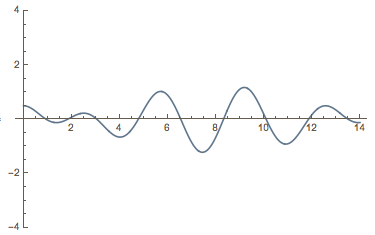
\includegraphics[height=2.5cm,width=5cm]{W05_DD1_Q2-1} 
\end{figure}

			\item \text{Q2-2} \begin{figure}[h!]
	\raggedright
		\graphicspath{{/Users/tylertrogden/Desktop/}}
		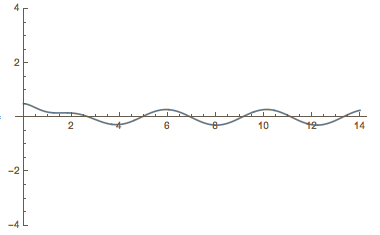
\includegraphics[height=2.5cm,width=5cm]{W05_DD1_Q2-2} 
\end{figure}

			\item \text{Q2-3} \begin{figure}[h!]
	\raggedright
		\graphicspath{{/Users/tylertrogden/Desktop/}}
		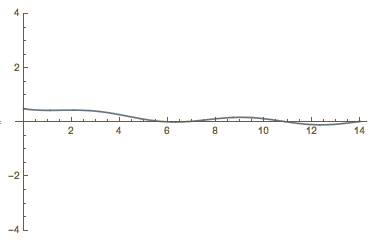
\includegraphics[height=2.5cm,width=5cm]{W05_DD1_Q2-3} 
\end{figure}

			\item \text{Q2-4} \begin{figure}[h!]
	\raggedright
		\graphicspath{{/Users/tylertrogden/Desktop/}}
		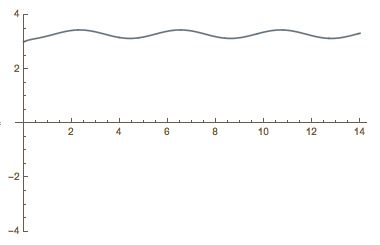
\includegraphics[height=2.5cm,width=5cm]{W05_DD1_Q2-4} 
\end{figure}

		\end{enumerate}
		
	\item \textbf{Change} to : ``Find the inverse Laplace Transform of the given F(s) function." 
	
	$F(s)=\frac{3}{(s-2)^2}$
		\begin{enumerate} 
			\item $f(t)=\frac{3}{\sqrt{2}}\sin{\sqrt{2}t}$
			\item $f(t)=3e^{2t}t^{2}$
			\item $f(t)=3e^{2t}t$ $\implies$ Correct
			\item $f(t)=3e^{2t}\sin{t}$
		\end{enumerate}
	
	\item \textbf{Keep.}
	
	\item \textbf{Keep.}
\end{enumerate}

\subsection*{DD2 Group Quiz}

\begin{enumerate}
	\item \textbf{Add.} ``A mass of 2 kg is attached to a spring with a spring constant of 100 $\frac{N}{m}$, it is suspended from the ceiling and hangs in equilibrium undisturbed (the system is subject to acceleration due to gravity). It is then driven by a periodic force, $f(t)=4\sin{7t}$, with air present so that the system experiences drag with a drag coefficient of 1 $\frac{kg}{s}$. Identify the model that most accurately represents this system."
		\begin{enumerate}
			\item $2y''+100y=4\sin{7t}+2g;\, y(0)=0,\, y'(0)=0$
			\item $y''+y'+50y=2\sin{7t}+g;\, y(0)=0,\, y'(0)=0$
			\item $2y''+y'+100y=4\sin{7t}+2g;\, y(0)=0,\, y'(0)=0$ $\implies$ \textbf{Correct}
			\item $y''+\frac{1}{2}y'+50y=0;\, y(0)=0,\, y'(0)=0$
		\end{enumerate}
	\item \textbf{Keep} (previously question 1). Please restate the first sentence of the question so that it reads as: ``An RLC circuit has a resistor with a resistance of 4 $\Omega$, an inductor with an inductance of 2 H, and a capacitor with a capacitance of 0.015 F, in series."
	
	\item \textbf{Keep} (previously question 2). Please reword to, ``Take the model from question 2 and use Mathematica to find and plot the solution. Select the graph that most accurately represents your work."
	
	\item \textbf{Keep} (previously question 3). Please fix the directions so that they read as: ``Find the Heaviside form of f(t)...".
	
	\item \textbf{Keep} (previously question 4). Please restate the question so that it is as follows: ``What is the Laplace Transform of $t\ u(t-2)$?"
	
	\item \textbf{Change} (previously question 5). ``Solve the following differential equation using the method of Laplace Transforms."
	
	$y''-2y'-3y=u(t-3);\, y(0)=2,\, y'(0)=0$
		\begin{enumerate}
			\item $y(t)=u(t-3)\left[\frac{e^{3(t-3)}}{12}+\frac{e^{-(t-3)}}{4}-\frac{1}{3}\right]+\frac{e^{3t}}{2}+\frac{3e^{-t}}{2}$ $\implies$ \textbf{Correct}
			\item $y(t)=u(t-3)\left[\frac{e^{3(t-3)}}{12}+\frac{e^{-(t-3)}}{4}-\frac{1}{3}\right]+\frac{e^{3t}}{2}-\frac{e^{-t}}{2}$
			\item $y(t)=u(t-3)\left[\frac{e^{3t}}{12}+\frac{e^{-t}}{4}-\frac{1}{3}\right]+\frac{e^{3t}}{2}+\frac{3e^{-t}}{2}$
			\item None of the above.
		\end{enumerate}
\end{enumerate}

\subsection*{DD3 Weekly Quiz}

\begin{enumerate}
	\item \textbf{Keep} but the correct answer is not present. Change answers to the following:
		\begin{enumerate}
			\item $y(t)=\frac{53}{50}e^{-t}+\frac{65}{50}e^{-t}-\frac{3}{54}\cos{3t}-\frac{2}{25}\sin{3t}$
			\item $y(t)=\frac{53}{50}e^{-t}+\frac{65}{50}te^{-t}-\frac{3}{54}\cos{3t}-\frac{2}{25}\sin{3t}$ $\implies$ \textbf{Correct}
			\item $y(t)=e^{-t}+te^{-t}$
			\item $y(t)=\frac{3}{50}e^{-t}+\frac{13}{10}te^{-t}-\frac{3}{54}\cos{3t}-\frac{2}{25}\sin{3t}$
		\end{enumerate}
	\item \textbf{Keep} but the correct answer is not present. Change answers to the following:
		\begin{enumerate}
			\item $y(t)=u(t-2)[\ \frac{2}{3}e^{-2t}+\frac{4}{3}e^{t}-2\ ]+\frac{1}{3}\ (e^{-2t}+2e^{t})$
			\item $y(t)=u(t-2)[\ \frac{2}{3}e^{4-2t}+\frac{4}{3}e^{t-2}-2\ ]+\frac{1}{3}\ (e^{-2t}+2e^{t})$ $\implies$ \textbf{Correct}
			\item $y(t)=u(t-2)[\ \frac{2}{3}e^{4-2t}+\frac{4}{3}e^{t-2}-2\ ]+\frac{1}{3}\ e^{-2 t}(-1 + e^{3 t})$
			\item None of the above.
		\end{enumerate}
	\item \textbf{Keep} and please make sure that an appropriate answer is $\implies$ $l(t)=\frac{1}{3}\ e^{-t}\sin{3t}$
	\item \textbf{Keep} and please make sure that an appropriate answer is $\implies$ $y(t)=\frac{1}{5}\ (e^{-2t}-\cos{t}+2\sin{t})$
	\item \textbf{Keep} and please make sure that an appropriate answer is $\implies$ $y(t)=\frac{1}{5}\ (9-9 e^{2 t}\cos{t} + 18 e^{2 t}\sin{t})$
	\item \textbf{Keep} please make sure that an appropriate answer is $\implies$ $y(t)=\frac{1}{12}\ (-\cos{3 t} + 13 e^{t}\cos{\sqrt{2} t} - \sin{3 t} - 
   5 \sqrt{2} e^{t} \sin{\sqrt{2} t})$
\end{enumerate}
\end{document}